\chapter{Manual de despliegue}
\label{cap:manual}

Este capítulo describe cómo instalar, configurar y ejecutar el sistema, qué
artefactos produce cada script y cómo interpretar los resultados. Este capítulo es una guía práctica de uso
paso a paso, pensada para que cualquier persona con el dataset descargado
pueda reproducir los resultados de esta memoria.

\section{Requisitos previos}
\label{sec:manual-requisitos}

La Tabla~\ref{tab:manual-requisitos} resume el software necesario para
ejecutar tanto el pipeline offline en Python como la aplicación web. El
proyecto se ha desarrollado y probado en Windows y macOS
(sección~\ref{sec:gestion-entorno}), sin dependencias específicas de
sistema operativo más allá de las propias de Python y Node.js.

\begin{table}[htp]
\centering
\caption{Requisitos previos para desplegar el sistema completo.}
\label{tab:manual-requisitos}
\renewcommand{\arraystretch}{1.25}
\begin{tabular}{|p{3.4cm}|p{9.4cm}|}
\hline
\rowcolor{gray!25}
\textbf{Requisito} & \textbf{Detalle} \\
\hline
Python & 3.11: versiones más recientes de Python no son
  compatibles con las versiones de las librerías usadas en este proyecto. \\
\hline
Node.js & 18 o superior, con \texttt{npm} incluido (necesario solo para la
  aplicación web). \\
\hline
Git & Cualquier versión reciente, para clonar el repositorio. \\
\hline
Espacio en disco & Al menos 60\,GB libres: el conjunto completo de la tarea
  \texttt{tracking} de SoccerNet (\emph{splits} train, test y challenge)
  ocupa unos 55\,GB una vez descomprimido. \\
\hline
Conexión a internet & Estable y sin límite de datos ajustado durante la
  descarga inicial del dataset, dado
  su tamaño. \\
\hline
\end{tabular}
\end{table}

No se requiere GPU: los algoritmos de tracking usados (ByteTrack, OC-SORT)
son clásicos y todo el pipeline se ha ejecutado sobre CPU sin que ello
supusiera una limitación relevante (sección~\ref{sec:gestion-entorno}).

\section{Instalación}
\label{sec:manual-instalacion}

\subsection{Obtención del código}

El código fuente está alojado en el repositorio de GitHub del proyecto:

\begin{lstlisting}[language=bash]
git clone https://github.com/cgaleam/Soccernet-Tracking-Analysis.git
cd Soccernet-Tracking-Analysis
\end{lstlisting}

Todas las rutas relativas del pipeline (\texttt{../SoccerNet/...}, usadas de
forma consistente en los scripts de \texttt{src/}) asumen que el dataset se
descarga como una carpeta hermana del repositorio, no dentro de él.

\subsection{Entorno Python}
\label{subsec:manual-venv}

El proyecto usa un entorno virtual estándar de Python, no \texttt{conda}
(problema P2, Tabla~\ref{tab:impl-problemas}):

\begin{lstlisting}[language=bash]
python3.11 -m venv venv_tfg

# macOS / Linux
source venv_tfg/bin/activate

# Windows (PowerShell)
venv_tfg\Scripts\Activate.ps1

pip install -r requirements.txt
\end{lstlisting}

\texttt{requirements.txt} fija las versiones exactas de todas las
dependencias, incluyendo \texttt{numpy==2.4.4}, \texttt{boxmot==10.0.43} y
\texttt{opencv-python==4.13.0.92}
. Existe una inconsistencia
conocida y documentada, \texttt{trackeval} no aparece listado explícitamente en
\texttt{requirements.txt} aunque el resto del pipeline lo importa
directamente. Si \texttt{pip install -r requirements.txt} no lo instala
como dependencia de otro paquete, instalarlo aparte con
\texttt{pip install trackeval}.

\subsection{Descarga del dataset SoccerNet}
\label{subsec:manual-dataset}

La descarga se realiza con el SDK oficial de SoccerNet, incluido en
\texttt{requirements.txt}:

\begin{lstlisting}[language=bash]
python src/utils/soccernet_download.py
\end{lstlisting}

Este script descarga los \emph{splits} train, test y challenge de las
tareas \texttt{tracking} y \texttt{tracking-2023} en una carpeta
\texttt{SoccerNet/} creada en paralelo al repositorio, reproduciendo la estructura
\texttt{SoccerNet/tracking/\{train,test,challenge\}/SNMOT-XXX/} que
consumen el resto de scripts del proyecto. A diferencia de otras tareas del
ecosistema SoccerNet que exigen solicitar acceso mediante un formulario
NDA (por ejemplo, los vídeos completos de partido), la tarea
\texttt{tracking} se descarga con una contraseña genérica de acceso
público, incluida en el propio SDK, sin gestión adicional por parte
del usuario. En la ejecución realizada durante este proyecto, la tarea
\texttt{tracking-2023} no llegó a descargar ningún dato (el propio SDK
informa de que ese \emph{split} concreto no estaba disponible en el
servidor en ese momento), sin que ello afecte al resto del pipeline, que
usa exclusivamente la tarea \texttt{tracking}.

\section{Estructura del repositorio}
\label{sec:manual-estructura}

La Tabla~\ref{tab:impl-estructura}
detalla la responsabilidad de cada paquete de \texttt{src/}. A efectos
prácticos de navegación, el árbol de directorios relevante tras completar
la instalación y una primera ejecución completa es el siguiente:

\begin{lstlisting}[language=bash]
Soccernet-Tracking-Analysis/
  src/
    visualizacion/        # scripts exploratorios iniciales
    tracking/             # ByteTrack, OC-SORT, ejecucion batch, export de video
    evaluation/           # seqmaps + evaluacion con TrackEval
    hyperparameter_study/
    metadata/             # equipos, heatmaps, homografia, posesion
    web_export/           # metadatos de OC-SORT + paquete de datos para la web
    utils/
  frontend/                # aplicacion web
  results_train/, results_test/          # .txt de tracking por secuencia
  results_hyperparam/                    # resultados del barrido + configuraciones optimas
  evaluation_train/, evaluation_test/    # salida de TrackEval
  evaluation_hyperparam/                 # resumen + graficas del estudio de hiperparametros
  metadata_output/                       # equipos, heatmaps, homografia, posesion
  videos/                                # videos anotados exportados
  memoria/                               # este documento
  requirements.txt
  venv_tfg/                              # entorno virtual
\end{lstlisting}

\texttt{results\_train/}, \texttt{evaluation\_train/} y el resto de
carpetas de salida no se incluyen en el repositorio: las genera cada script
la primera vez que se ejecuta.

\section{Ejecución del pipeline de tracking}
\label{sec:manual-tracking}

Los scripts de \texttt{src/tracking/} cubren dos casos de uso distintos:
explorar una única secuencia con un algoritmo concreto, o procesar un
\emph{split} completo con ambos algoritmos (sección~\ref{sec:implementacion-tracking}).

Para explorar una única secuencia, \texttt{bytetracker\_alg.py} y
\texttt{sort\_alg.py} no aceptan argumentos
de línea de comandos: la secuencia a procesar se fija editando la variable
\texttt{base\_path} al principio del fichero antes de ejecutarlo.

\begin{lstlisting}[language=bash]
# Editar antes de ejecutar: base_path = "../SoccerNet/tracking/train/SNMOT-XXX/"
python src/tracking/bytetracker_alg.py
python src/tracking/sort_alg.py
\end{lstlisting}

Para reproducir los resultados de esta memoria, el flujo real es la
ejecución batch sobre el \emph{split} completo, que sí recorre todas las
secuencias automáticamente:

\begin{lstlisting}[language=bash]
python src/tracking/run_all_train.py   # -> results_train/{bytetracker,ocsort}/
python src/tracking/run_all_test.py    # -> results_test/{bytetracker,ocsort}/
\end{lstlisting}

Cada ejecución tarda del orden de varias horas sobre CPU, al procesar las
57 secuencias de train o las 49 de test con ambos algoritmos
frame a frame. Para exportar un vídeo anotado de una secuencia concreta
(por defecto, SNMOT-076 de train):

\begin{lstlisting}[language=bash]
python src/tracking/export/export_bytetracker.py   # -> videos/SNMOT-076_bytetracker.mp4
python src/tracking/export/export_sort.py           # -> videos/SNMOT-076_ocsort.mp4
\end{lstlisting}

\section{Ejecución de la evaluación}
\label{sec:manual-evaluacion}

\texttt{TrackEval} necesita un fichero \emph{seqmap} que le indique qué
secuencias evaluar, que debe generarse antes de la evaluación propiamente
dicha:

\begin{lstlisting}[language=bash]
python src/evaluation/seqmpas_creation_train.py
python src/evaluation/seqmaps_creation_test.py
python src/evaluation/evaluate_train.py   # -> evaluation_train/
python src/evaluation/evaluate_test.py    # -> evaluation_test/
\end{lstlisting}

Cada carpeta de salida contiene, por algoritmo y secuencia, un
\texttt{pedestrian\_summary.txt} con las columnas de HOTA, HOTA(0), DetA,
AssA, MOTA e IDF1 usadas en la comparativa del
capítulo~\ref{cap:pruebas}.

\section{Ejecución del estudio de hiperparámetros}
\label{sec:manual-hiperparametros}

\begin{lstlisting}[language=bash]
python src/hyperparameter_study/hyperparam_bytetracker.py  # -> results_hyperparam/bytetracker/
python src/hyperparameter_study/hyperparam_ocsort.py       # -> results_hyperparam/ocsort/
python src/hyperparameter_study/summarize_hyperparam.py    # -> evaluation_hyperparam/summary_table.csv y /plots/
python src/hyperparameter_study/bytetracker_optimal.py     # -> results_hyperparam/bytetracker/bytetracker_optimal/
python src/hyperparameter_study/ocsort_optimal.py          # -> results_hyperparam/ocsort_optimal/
\end{lstlisting}

Los dos primeros scripts varían un hiperparámetro a la vez sobre el
\emph{split} de test, manteniendo el resto en su valor base
(sección~\ref{sec:implementacion-hiperparametros}); cada barrido completo
tarda igualmente del orden de horas. \texttt{summarize\_hyperparam.py} debe
ejecutarse después de ambos barridos, ya que lee sus resultados y produce
la tabla y las gráficas comparativas reutilizadas en el
capítulo~\ref{cap:pruebas}. Los dos últimos scripts no forman parte del
barrido: ejecutan y evalúan cada algoritmo una única vez con la
configuración óptima ya determinada, y son los que alimentan tanto el
pipeline de metadatos como la aplicación web.

\section{Ejecución del pipeline de metadatos}
\label{sec:manual-metadatos}

Todos los scripts de \texttt{src/metadata/} parten de
\texttt{results\_hyperparam/bytetracker/bytetracker\_optimal/}
 y deben ejecutarse en este
orden, ya que la clasificación de equipos es una dependencia de los
mapas de calor por equipo y de la posesión:

\begin{lstlisting}[language=bash]
python src/metadata/team_classification.py       # -> metadata_output/teams/*_teams_final.csv
python src/metadata/team_visualization.py         # -> metadata_output/teams/*_frame*.png
python src/metadata/heatmap_field.py               # -> metadata_output/heatmaps/*_heatmap_field.png
python src/metadata/heatmap_by_team.py             # -> metadata_output/heatmaps/*_heatmap_by_team.png
python src/metadata/distance_homography_demo_116.py
python src/metadata/distance_homography_demo_118.py
python src/metadata/heatmap_homography_demo_116.py
python src/metadata/heatmap_homography_demo_118.py
python src/metadata/ball_possesion.py              # -> metadata_output/possession/
\end{lstlisting}

\texttt{general\_heatmap.py} es la primera versión del mapa de calor
general y se
conserva en el repositorio a título documental, pero no forma parte del
flujo actual: \texttt{heatmap\_field.py} la sustituye por completo.
\texttt{distance\_homography\_demo\_*.py} y
\texttt{heatmap\_homography\_demo\_*.py} solo existen para SNMOT-116 y
SNMOT-118, las dos secuencias con calibración de homografía manual.

Para generar el mismo conjunto de metadatos sobre la configuración óptima
de OC-SORT, necesario para el selector de algoritmo de la aplicación
web, no para el pipeline principal, que solo usa ByteTrack, el paquete
\texttt{src/web\_export/} reproduce esta misma lógica parametrizada por
algoritmo en lugar de duplicar cada
script.


\section{Manual de la aplicación web}
\label{sec:manual-web}

\subsection{Generación del paquete de datos}

La aplicación web no recalcula nada: consume un paquete de artefactos
estáticos que debe
generarse antes de arrancarla, una vez completados los pasos anteriores
para ambos algoritmos:

\begin{lstlisting}[language=bash]
python -m src.web_export.export_bundle
# -> frontend/public/data/{videos,images}/, sequences.json, global_metrics.json
\end{lstlisting}

Este paso reescribe por completo la carpeta \texttt{frontend/public/data/} y debe repetirse cada vez que
cambien los resultados de tracking, evaluación o metadatos que consume.

\subsection{Instalación y ejecución del frontend}

\begin{lstlisting}[language=bash]
cd frontend
npm install

npm run dev      # servidor de desarrollo, http://localhost:5173
npm run build     # build estatico
npm run preview   # sirve el build de dist/ en local para verificarlo
\end{lstlisting}

\texttt{npm run dev} recarga automáticamente al editar el código de
\texttt{frontend/src/}, pero no vigila \texttt{frontend/public/data/}: si
se regenera el paquete de datos con \texttt{export\_bundle.py} mientras el
servidor de desarrollo está en marcha, hay que reiniciarlo para que recoja
los ficheros nuevos. El build de producción
(\texttt{npm run build}) genera un sitio completamente estático en
\texttt{frontend/dist/}, con rutas relativas
(\texttt{base: './'} en \texttt{vite.config.ts}), desplegable en cualquier
alojamiento estático o servible directamente en local.

\subsection{Uso de la interfaz}
\label{subsec:manual-uso-interfaz}

La aplicación se organiza en dos pestañas,
pensadas para responder dos preguntas distintas: \enquote{¿qué algoritmo
rinde mejor en general?} y \enquote{¿qué ha pasado exactamente en esta
secuencia concreta?}. Las Figuras~\ref{fig:manual-web-comparativa}
a~\ref{fig:manual-web-118} son capturas reales de la aplicación en
ejecución sobre el paquete de datos descrito en la
sección~\ref{subsec:impl-web-bundle}, y se usan a continuación para
detallar, panel a panel, qué permite consultar cada pestaña.

\paragraph{Comparativa de algoritmos.} Esta pestaña
(Figura~\ref{fig:manual-web-comparativa}) no requiere seleccionar nada:
muestra directamente, para entrenamiento y test por separado, la tabla de
métricas de ambos algoritmos, el gráfico de
barras que contrasta HOTA integrada frente a HOTA(0), la discrepancia
metodológica central de este proyecto
(sección~\ref{subsec:impl-hota-vs-hota0}), la tabla con la configuración
óptima de hiperparámetros de cada algoritmo, y las gráficas del estudio
de sensibilidad del
capítulo~\ref{cap:pruebas}.

\begin{figure}[htp]
\centering
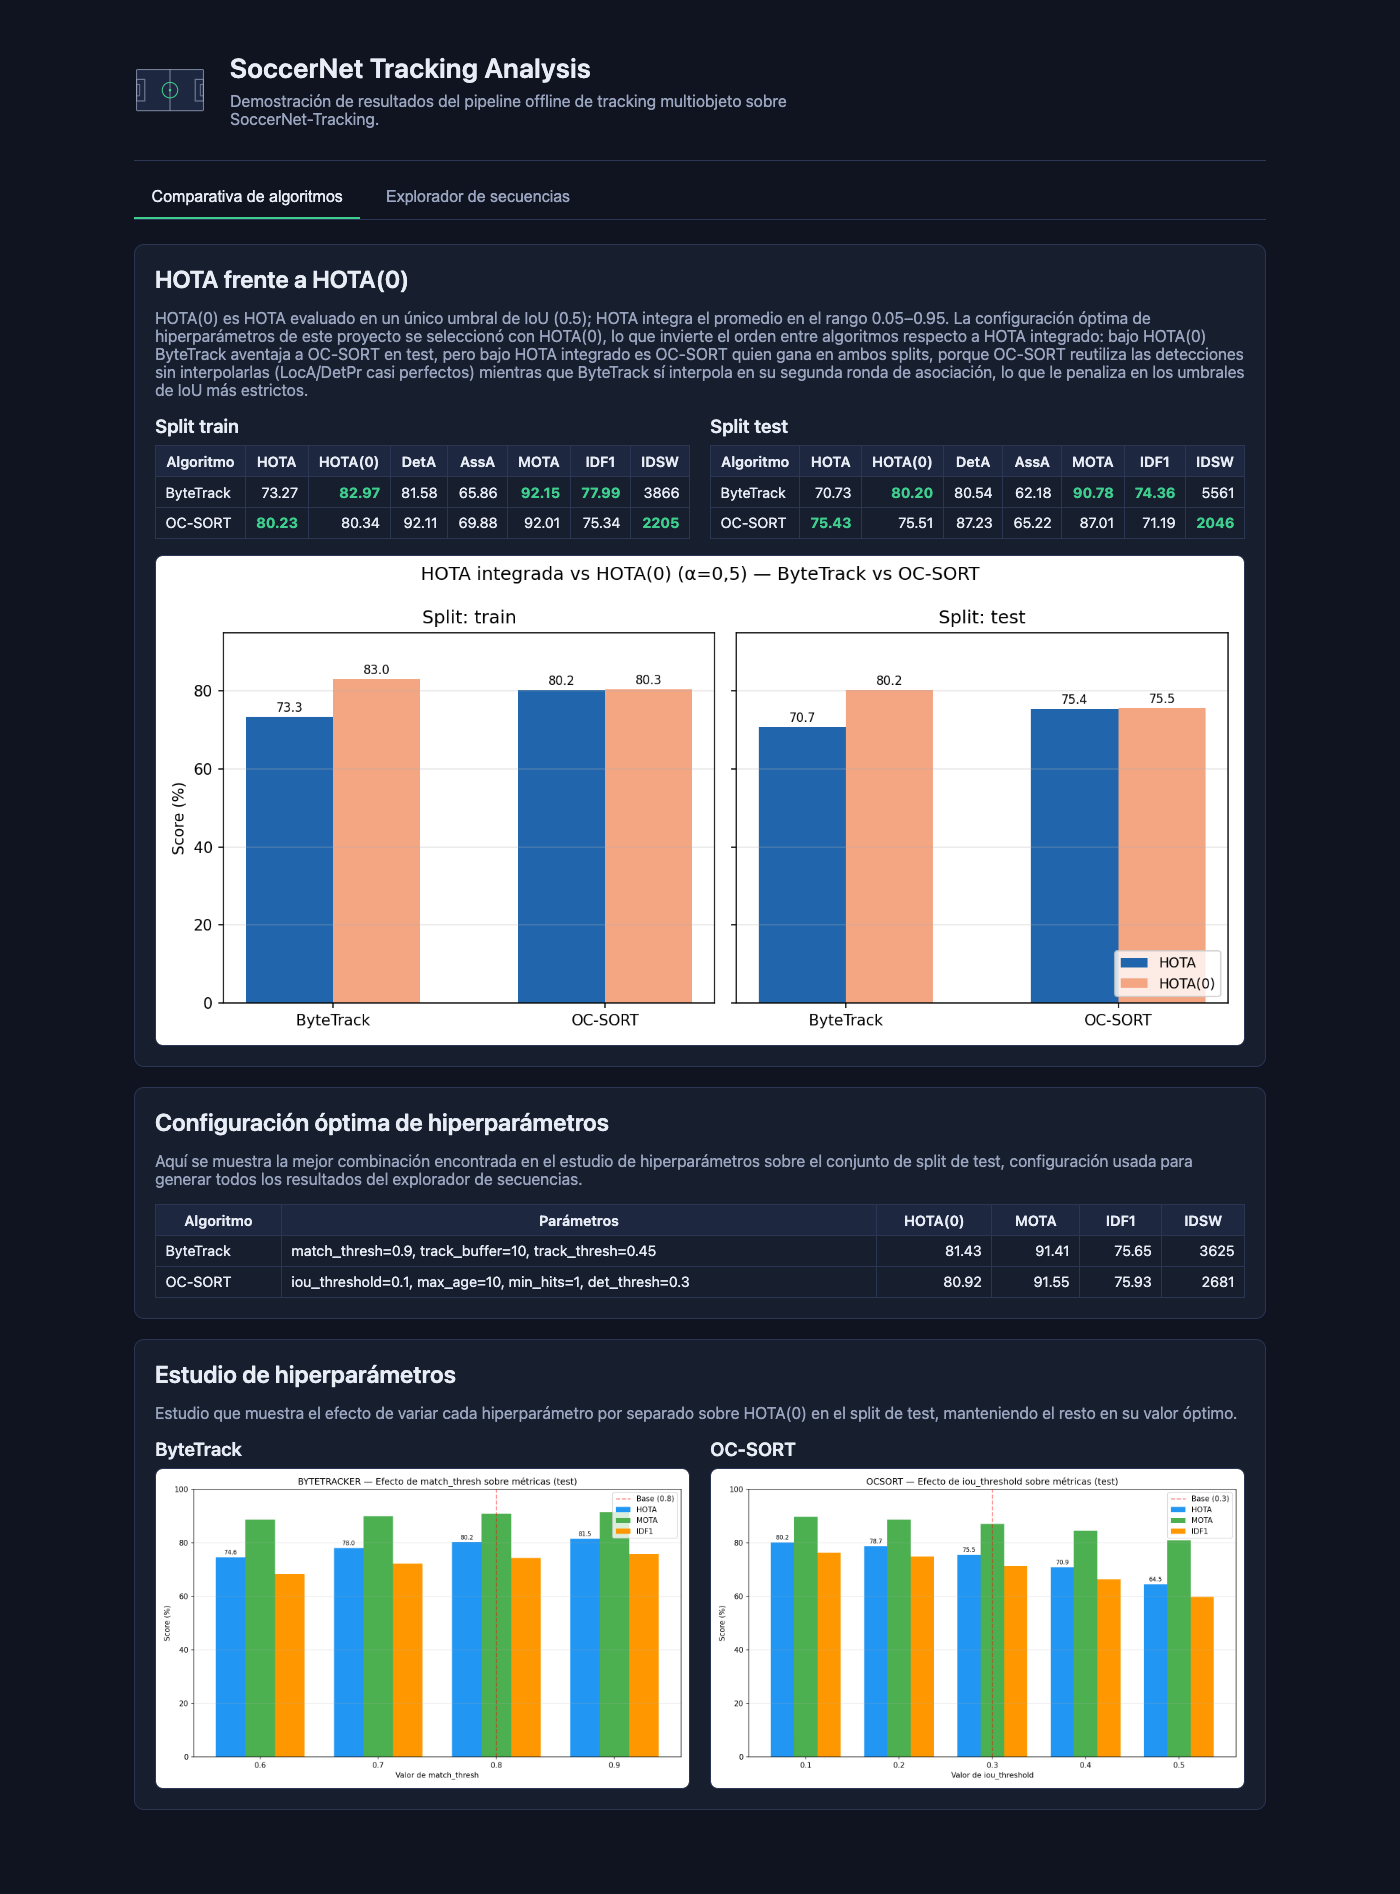
\includegraphics[height=0.8\textheight, keepaspectratio]{figures/manual_web_comparativa.png}
\caption[Pestaña \enquote{Comparativa de algoritmos}]{Pestaña
\enquote{Comparativa de algoritmos}: tabla de métricas por \emph{split},
gráfico HOTA frente a HOTA(0), configuración óptima de hiperparámetros y
gráficas de sensibilidad.}
\label{fig:manual-web-comparativa}
\end{figure}

\FloatBarrier

\paragraph{Explorador de secuencias: selección y vídeo.} Esta pestaña
(Figuras~\ref{fig:manual-web-116} a~\ref{fig:manual-web-118}) exige
elegir primero una secuencia (SNMOT-116/117/118) y un algoritmo
(ByteTrack u OC-SORT) mediante los selectores de chips de la parte
superior; el resto de la pestaña se actualiza automáticamente con los
datos de esa combinación concreta, sin recargar la página. El panel de
vídeo reproduce el tramo correspondiente con las cajas delimitadoras
superpuestas, coloreadas por equipo, con el identificador de tracking
de cada jugador y el balón resaltado en un color distinto mediante los
controles estándar de un reproductor, lo que permite comprobar visualmente, frame
a frame si es necesario, la calidad real del tracking sobre el que se
calcula el resto de metadatos.

\paragraph{Clasificación de equipos y posesión.} Debajo del vídeo, el
panel de \textbf{equipos} muestra cuántos jugadores se han clasificado y
el reparto entre Equipo~0 y Equipo~1 para esa combinación concreta, junto con la nota de limitación
sobre el árbitro. El panel de
\textbf{posesión}, a su lado, muestra el porcentaje de posesión de cada
equipo estimado por proximidad al balón.

\paragraph{Mapas de calor y homografía.} El panel de \textbf{mapas de
calor} permite comparar visualmente la ocupación del campo, tanto
general como separada por equipo, sobre la misma escala de color. Cuando la secuencia dispone de
calibración de homografía real,
un panel adicional de \textbf{homografía} muestra el mapa de calor
calibrado en metros reales y una tabla con el top-5 de jugadores por
distancia recorrida, junto con su velocidad media y de pico
(sección~\ref{subsec:diseno-homografia}). La
Figura~\ref{fig:manual-web-117} muestra precisamente el caso en que este
panel no está disponible, con la nota explícita que evita que la
ausencia de datos se confunda con un error de carga.

\begin{figure}[htp]
\centering
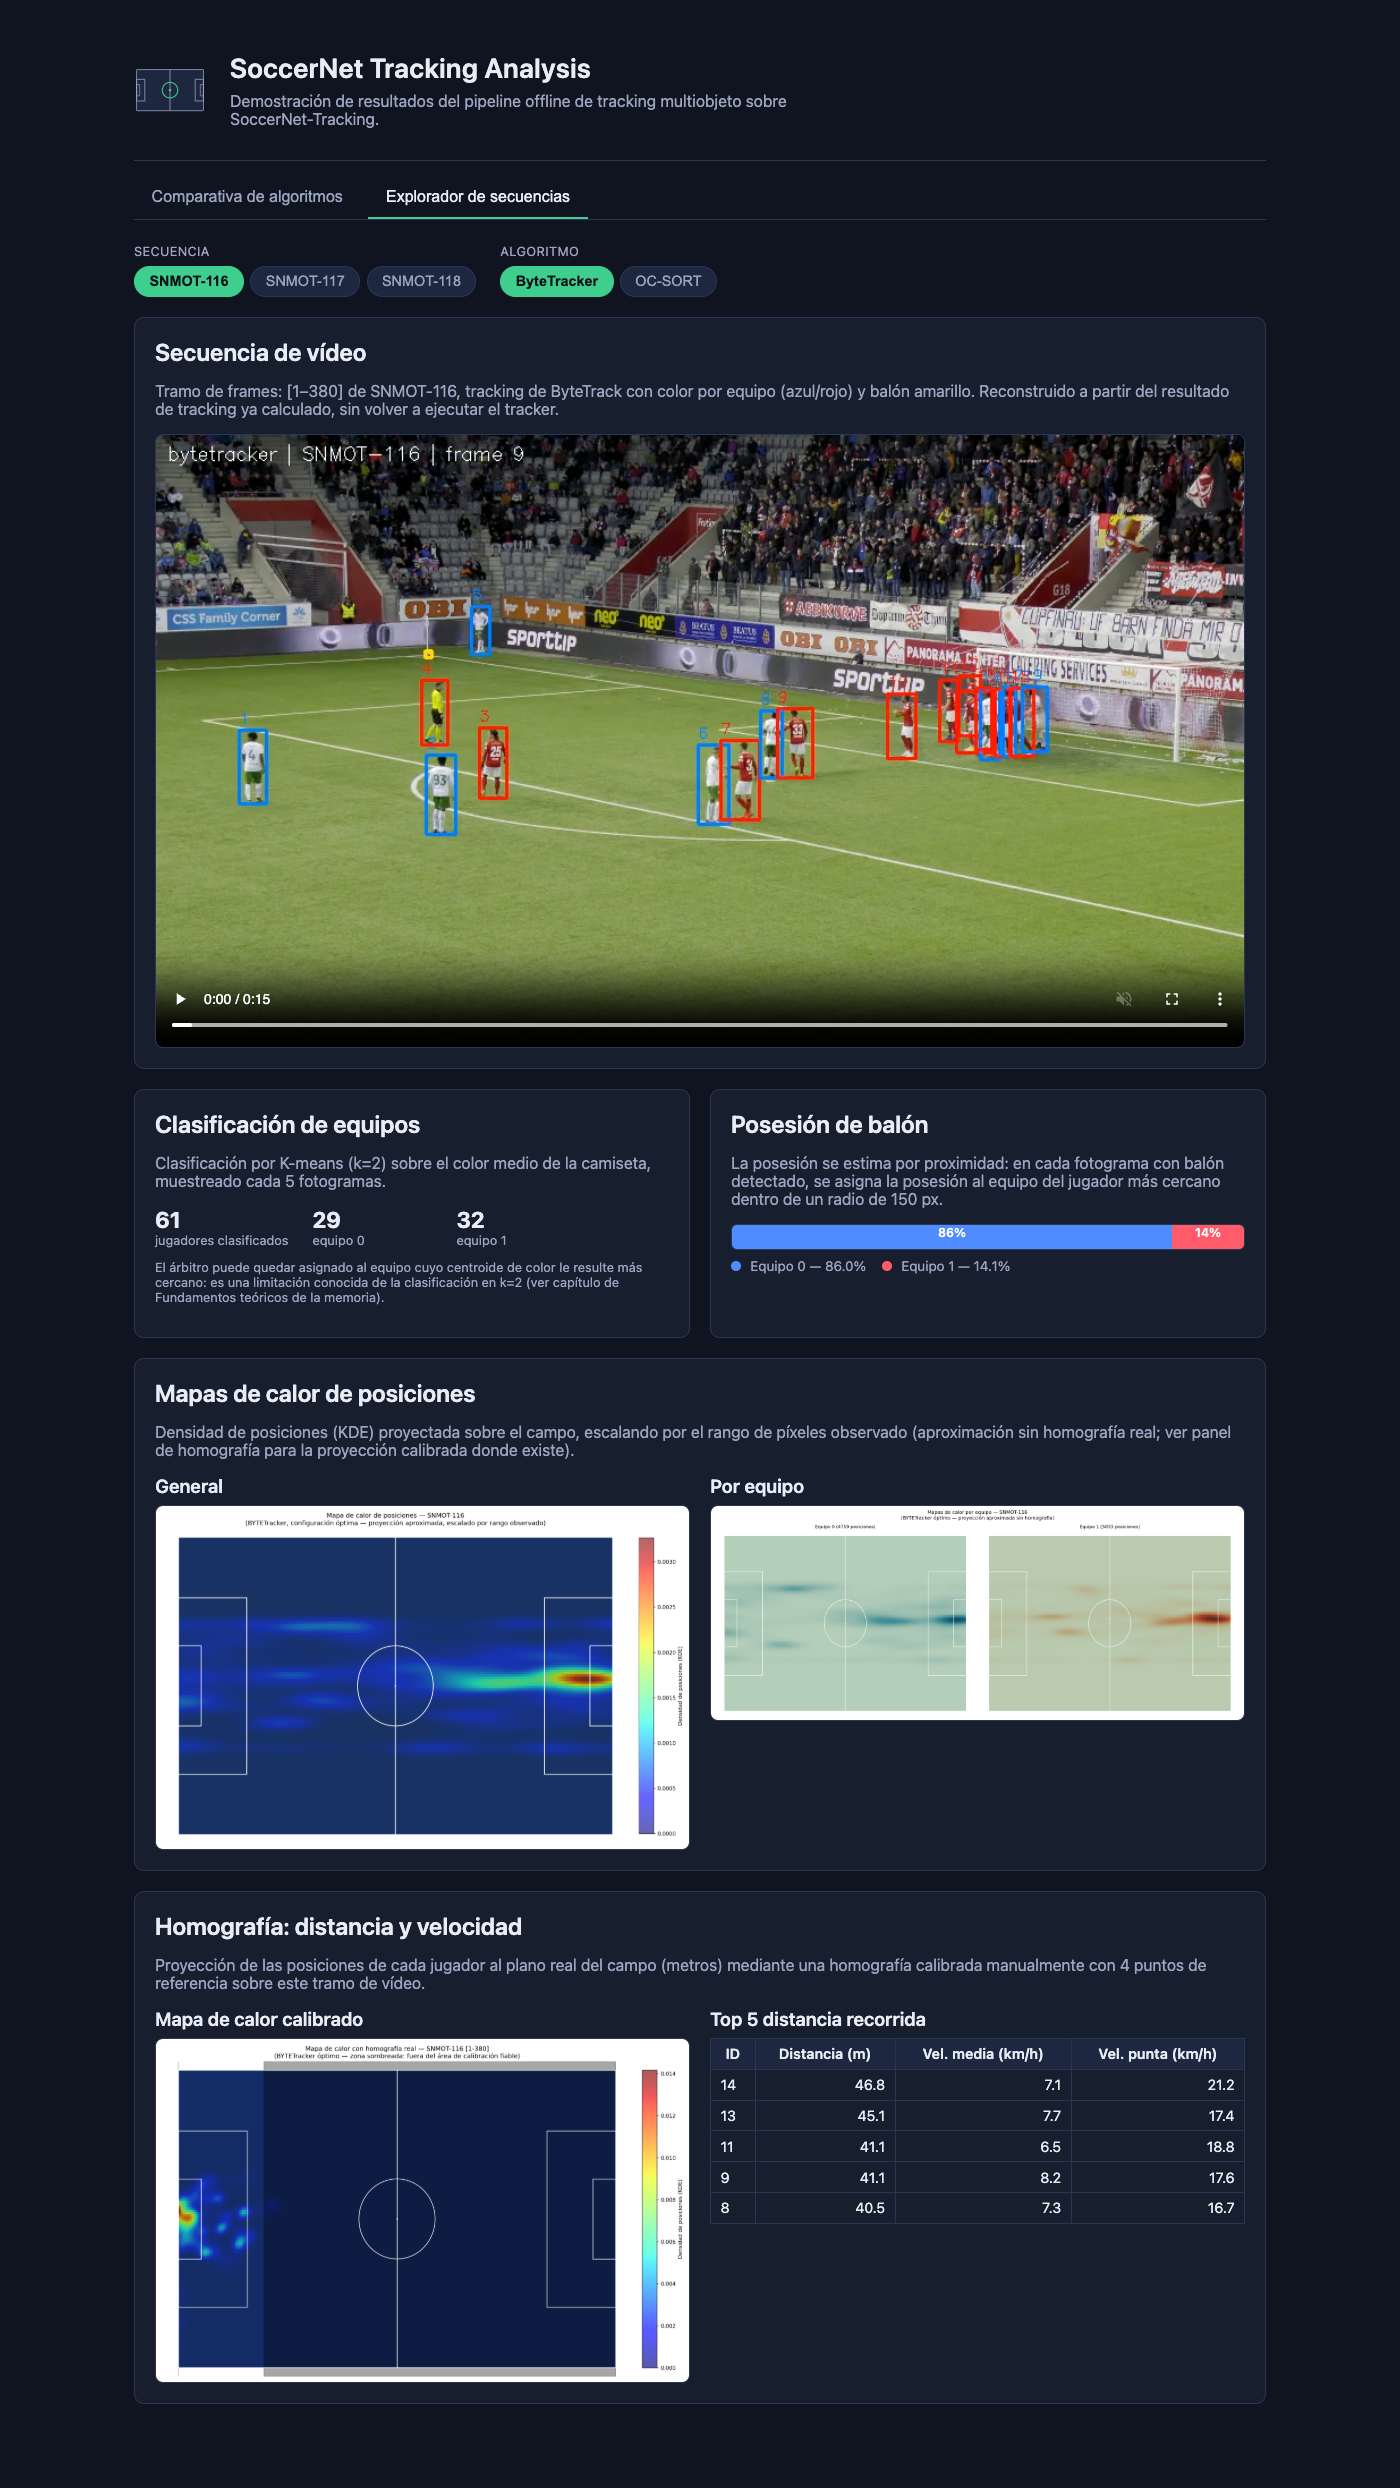
\includegraphics[height=0.8\textheight, keepaspectratio]{figures/manual_web_explorador_116.png}
\caption{Pestaña \enquote{Explorador de secuencias} con SNMOT-116 y
ByteTrack.}
\label{fig:manual-web-116}
\end{figure}

\FloatBarrier

\begin{figure}[htp]
\centering
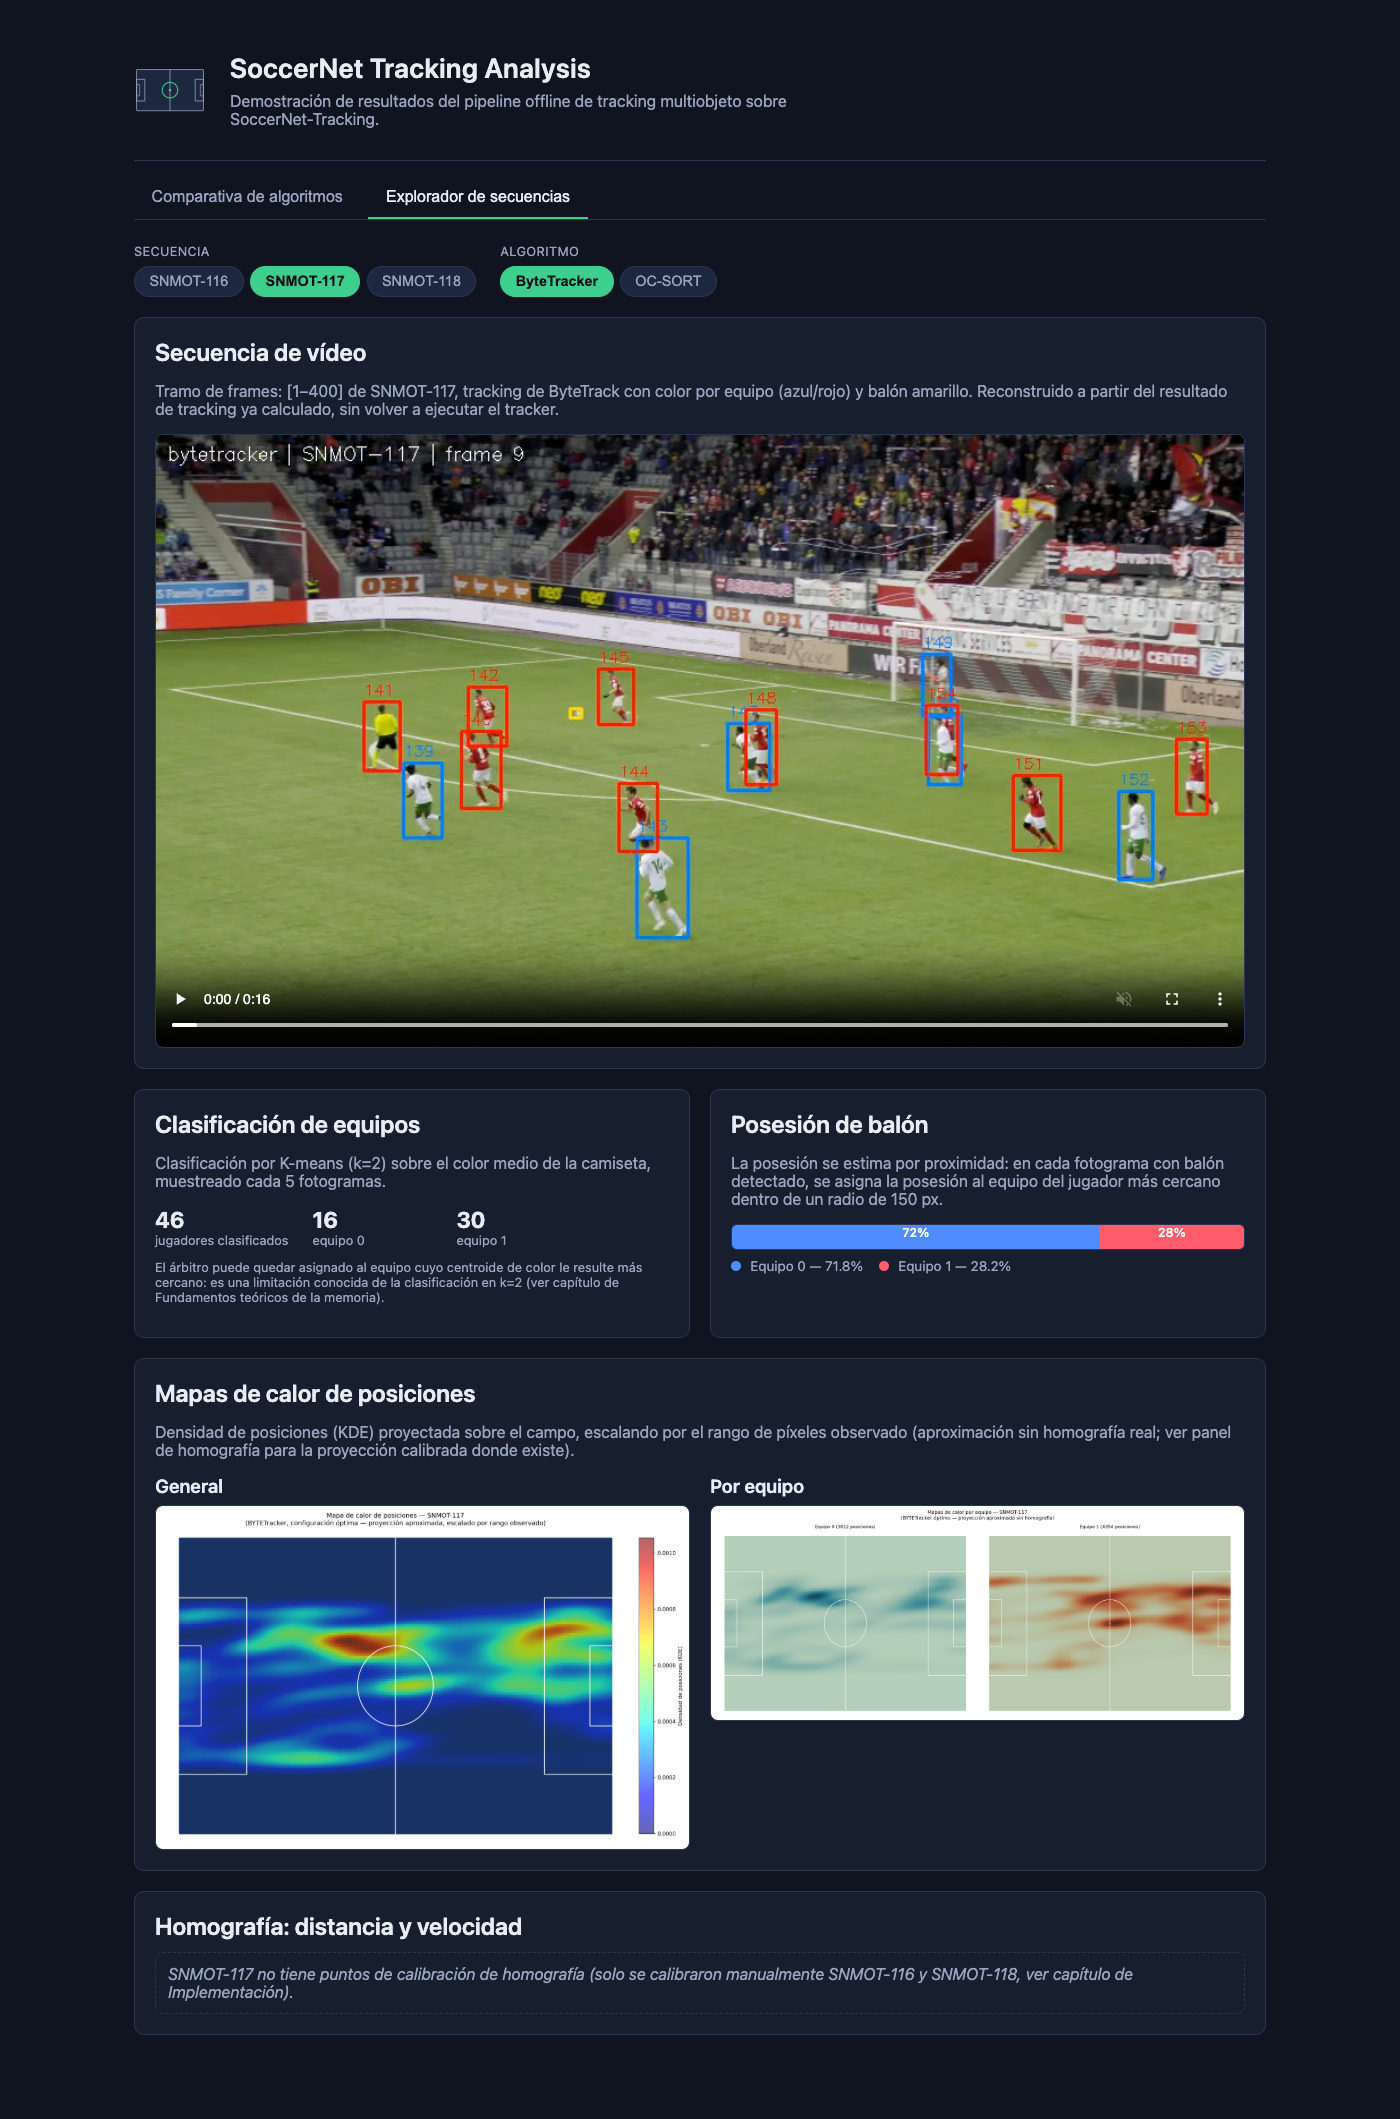
\includegraphics[height=0.8\textheight, keepaspectratio]{figures/manual_web_explorador_117.png}
\caption{SNMOT-117 con ByteTrack.}
\label{fig:manual-web-117}
\end{figure}

\FloatBarrier

\begin{figure}[htp]
\centering
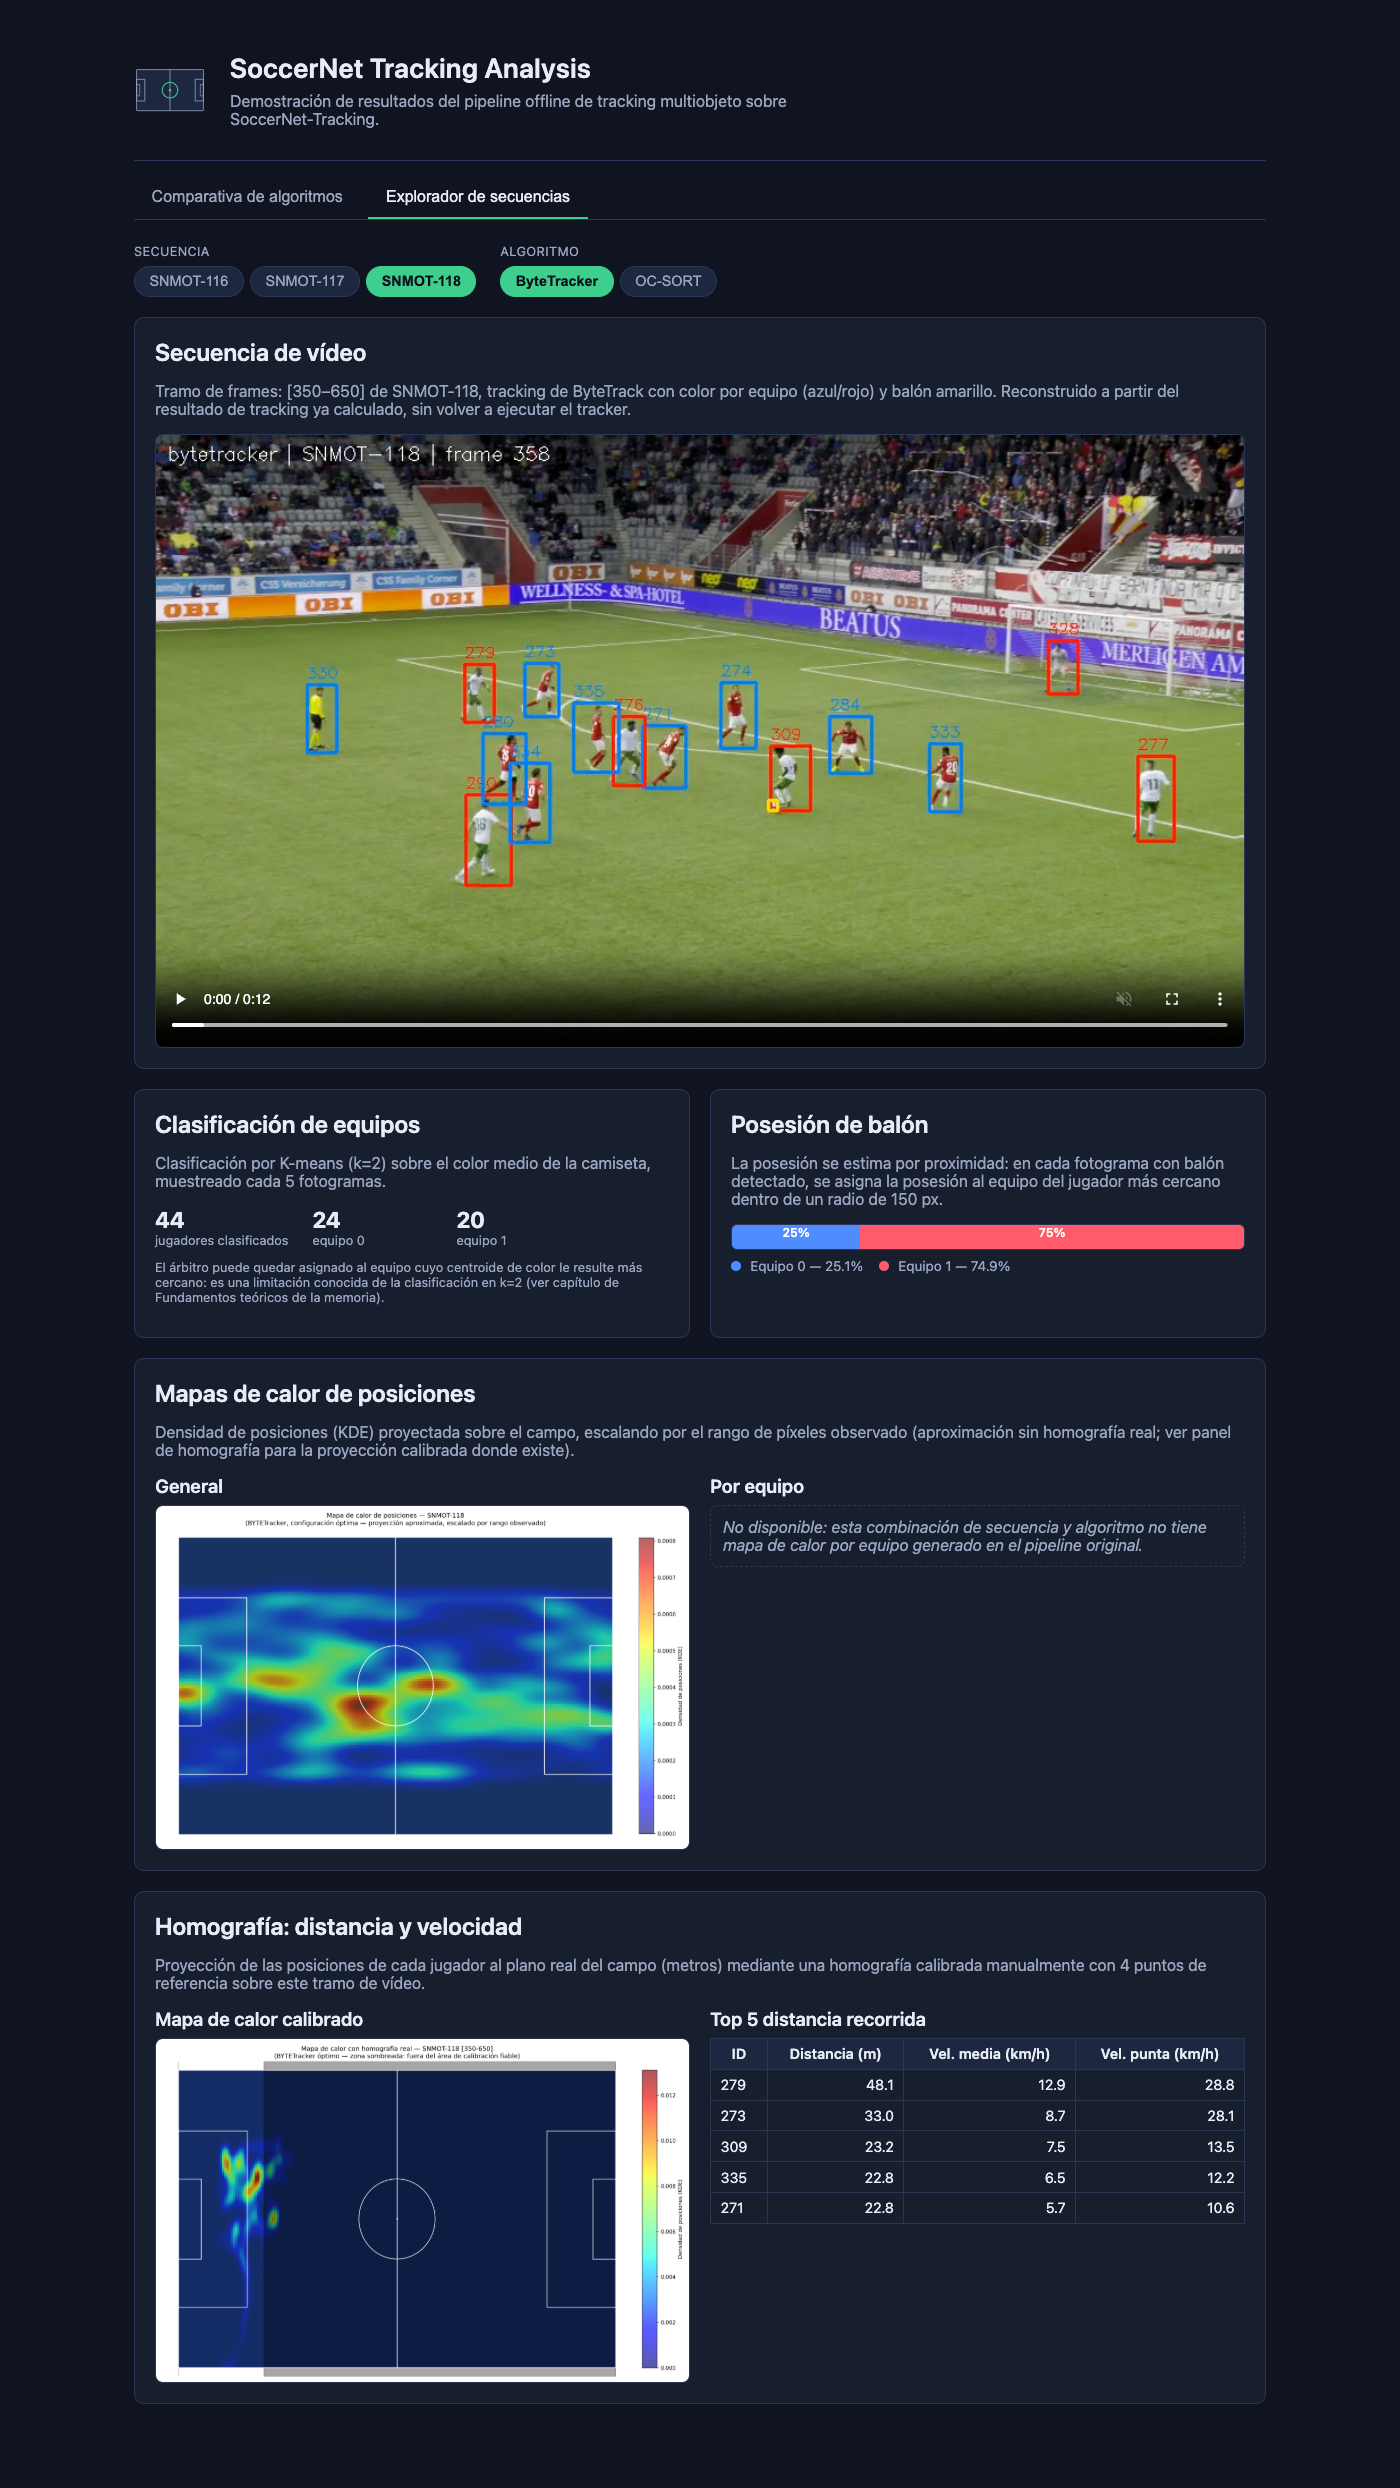
\includegraphics[height=0.8\textheight, keepaspectratio]{figures/manual_web_explorador_118.png}
\caption{SNMOT-118 con ByteTrack.}
\label{fig:manual-web-118}
\end{figure}

\section{Problemas frecuentes}
\label{sec:manual-problemas}

La Tabla~\ref{tab:manual-problemas} recoge, de forma complementaria, los
problemas más probables al desplegar el sistema desde cero siguiendo este
manual, con su causa y solución.

\begin{table}[htp]
\centering
\caption{Problemas frecuentes al desplegar el sistema y su solución.}
\label{tab:manual-problemas}
\renewcommand{\arraystretch}{1.2}
\footnotesize
\begin{tabular}{|p{4.6cm}|p{4.0cm}|p{4.5cm}|}
\hline
\rowcolor{gray!25}
\textbf{Síntoma} & \textbf{Causa} & \textbf{Solución} \\
\hline
\texttt{FileNotFoundError} al leer secuencias del dataset &
  El dataset no está en \texttt{../SoccerNet} relativo al repositorio &
  Clonar el repositorio y descargar el dataset como carpetas hermanas
  (sección~\ref{subsec:manual-dataset}) \\
\hline
Un script de \texttt{src/tracking/} o \texttt{src/metadata/} procesa
  siempre la misma secuencia & La secuencia está hardcodeada en una
  variable al principio del fichero (\texttt{base\_path},
  \texttt{SEQUENCE}) & Editar esa variable antes de ejecutar, o usar los
  scripts \texttt{run\_all\_*.py} para procesar el split completo \\
\hline
\texttt{ModuleNotFoundError: trackeval} al evaluar &
  \texttt{trackeval} no quedó instalado como dependencia transitiva &
  \texttt{pip install trackeval} (sección~\ref{subsec:manual-venv}) \\
\hline
\texttt{heatmap\_by\_team.py} o \texttt{ball\_possesion.py} fallan o dan
  resultados vacíos & No se ejecutó antes \texttt{team\_classification.py}
  para ese algoritmo & Respetar el orden de ejecución de la
  sección~\ref{sec:manual-metadatos} \\
\hline
Los vídeos generados por \texttt{export\_bundle.py} no se reproducen en el
  navegador & \emph{Fourcc} de OpenCV no soportado por navegadores
  (problema P17) & Ya corregido en el código del proyecto
  (\emph{fourcc} \texttt{avc1}); si se modifica el script, mantener ese
  \emph{fourcc} \\
\hline
La pestaña \emph{Explorador de secuencias} no refleja cambios recientes en
  los datos & \texttt{npm run dev} no vigila
  \texttt{frontend/public/data/} & Reiniciar el servidor de desarrollo
  tras regenerar el paquete de datos \\
\hline
\end{tabular}
\end{table}
